% CREATED BY DAVID FRISK, 2015
\chapter{Methods}


This chapter will describe methods and definitions of generating guidelines for brickwork on a surface that is a result of form finding. Definitions and procedure will be derived from the theory described in the previous chapter.   


\section{General}

The method will be based on geodesic coordinates and polar geodesic coordinates on a surface that has been described in \ref{sec:geoCord}. The main idea is to make a discrete formulation of the continuous definition of geodesics and in extension a discrete formulation of the geodesic coordinates. This will be implemented on a continuous surface using a discrete solver for dynamic problems, called dynamic relaxation, describe in section \ref{DR}. This will be implemented in a parametric design environment and part of a parametric design scheme described in \ref{dScheme}. The process and generation of geodesic coordinates will be described in the following chronological order of the implementation:
\vspace{5mm}
\begin{enumerate}
\item Form Finding, generate a form that fulfills equilibrium.
\item Generation of geodesic points on the surface.
\item From the geodesic points orthogonal trajectories will be constructed 
\end{enumerate}
\vspace{5mm}
The implementation is a bit different between the two types of geodesic coordinates but the main idea is similar.

\section{Discrete definitions}
This section will describe how this thesis interprets the continuous definitions in Classical Differential geometry to Discrete definitions. 
\subsection{Definition of discrete geodesic points}  \label{geopoint}


The continuous definition of a geodesic curve is that in each point along the curve the geodesic curvature is zero, i.e curve can only be curved in the normal direction. This could be interpreted as the tangent of the curve and the normal forming a plane. For a discrete definition one can imagine three points on a surface where the points are connected through two vectors,A and B, starting in the middle point, see figure below. If the normal of the middle point and the two vectors lies in the same plane the middle point is defined as a geodesic point. This means that the cross product of A and B is orthogonal to the normal and the projection on the normal would be zero, i.e the geodesic component is zero. And for a small enough distance on the surface a collection of geodesic points will form a geodesic curve.

\begin{figure}[H]
\centering
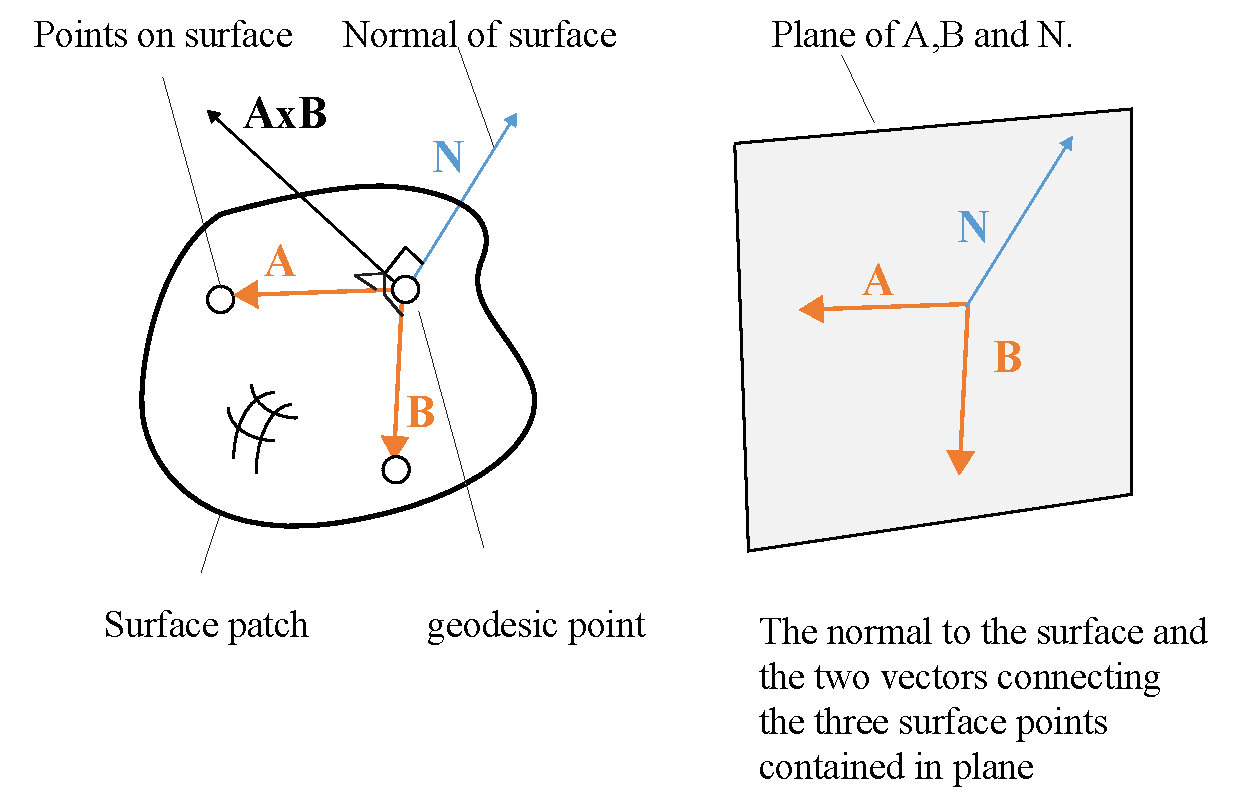
\includegraphics[width = 0.8\linewidth ]{figure/Method/defintionGeodeiscPoint.pdf}
\caption{http://web.mit.edu/hyperbook/Patrikalakis-Maekawa-Cho/node29.html}
\end{figure}

\subsubsection{Physical interpretation} \label{physdef}

Making a physical interpretation of the geodesic point is by defining a discrete curve as a set of connected springs. The springs are of the same initial length with a pre-tension, that is the same for all springs, is applied in the springs. Isolating the node one will find a spring force in the direction of the connected springs. Adding these two forces results in a resultant force in that node. When the resultant force can be described in  the normal of the surface in that point, the geodesic force component is zero. This is the physical definition of a geodesic point which equivalent the discrete defintion above.

\begin{figure}[H]
\centering
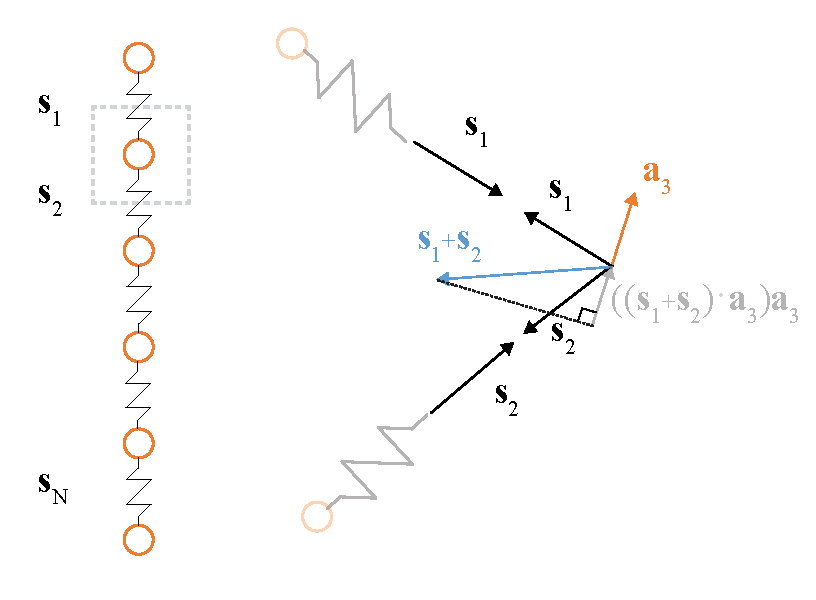
\includegraphics[width = 0.8\linewidth ]{figure/Method/GeodesicDR.pdf}
\caption{http://web.mit.edu/hyperbook/Patrikalakis-Maekawa-Cho/node29.html}
\end{figure}

\subsection{Definition of discrete curves}




\subsection{Definition of discrete geodesic coordinates}

There are, as mentioned, two types of geodesic coordinates:

\begin{enumerate}
\item General geodesic coordinates
\item Polar geodesic coordinates
\end{enumerate}

The main properties of a geodesic coordinate system is that it is formed of two sets of curves, the first is geodesics and the second is orthogonal trajectories that intersects the geodesics at right angles with an equal distance along the geodesics. In this section discrete equivalents definitions of the continuous definition will be made. These definitions require the discrete definition of geodesic points described in  \ref{geopoint}.\\

One important assumption for ensuring the discrete definitions in this thesis that will be applied to both is following statement by Struik regarding continuous geodesic coordinates:

\vspace{5mm}
\textit{ If geodesics be drawn orthogonal to a curve C, and segments of equal length be measured upon them from C, then the locus of their end points is an orthogonal trajectory of the geodesics.} 
\vspace{5mm}

For continuous differential geometry it means that we only need to find one orthogonal trajectory this a reference that can be used to find the next orthogonal trajectory. In this section we will describe what this reference is for both of these discrete cases.


\begin{figure}[H]
\centering
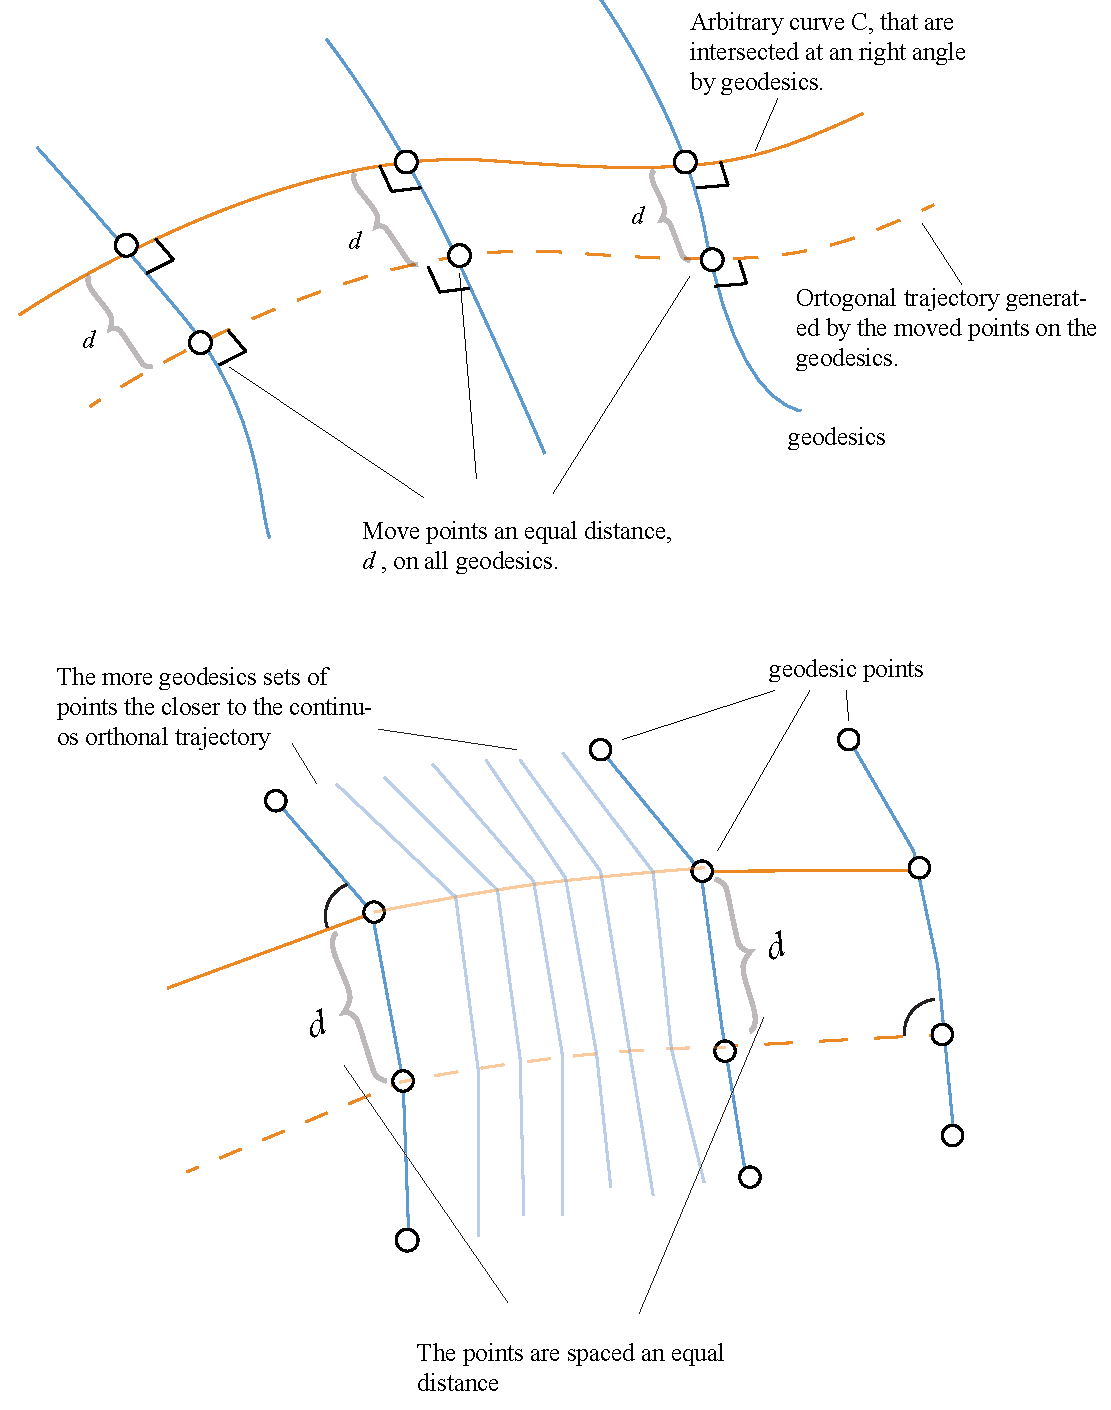
\includegraphics[width = 0.8\linewidth ]{figure/Method/geodesicDefintion.pdf}
\caption{http://web.mit.edu/hyperbook/Patrikalakis-Maekawa-Cho/node29.html}
\end{figure}


\subsubsection{Definition of discrete Polar geodesic coordinates}

The main difference is between polar and general geodesic coordinates is that in the polar coordinates the geodesics has its origin in the same point, the pole, and radially distribute from that point. The pole will play an important part for the discrete definition since the continuous definition states that at an equal distance along all geodesics we will find an orthogonal trajectory measured from the pole, see figure below.  Applying the same logic to a set of geodesic points, i.e the geodesic points are distributed at an equal distance from the pole and adjacent points as in figure below, the trajectories will not necessarily be orthogonal. This definition states that for a sufficient number of sets of geodesic points the trajectories will converge towards a continuous orthogonal trajectory. 

\begin{figure}[H]
\centering
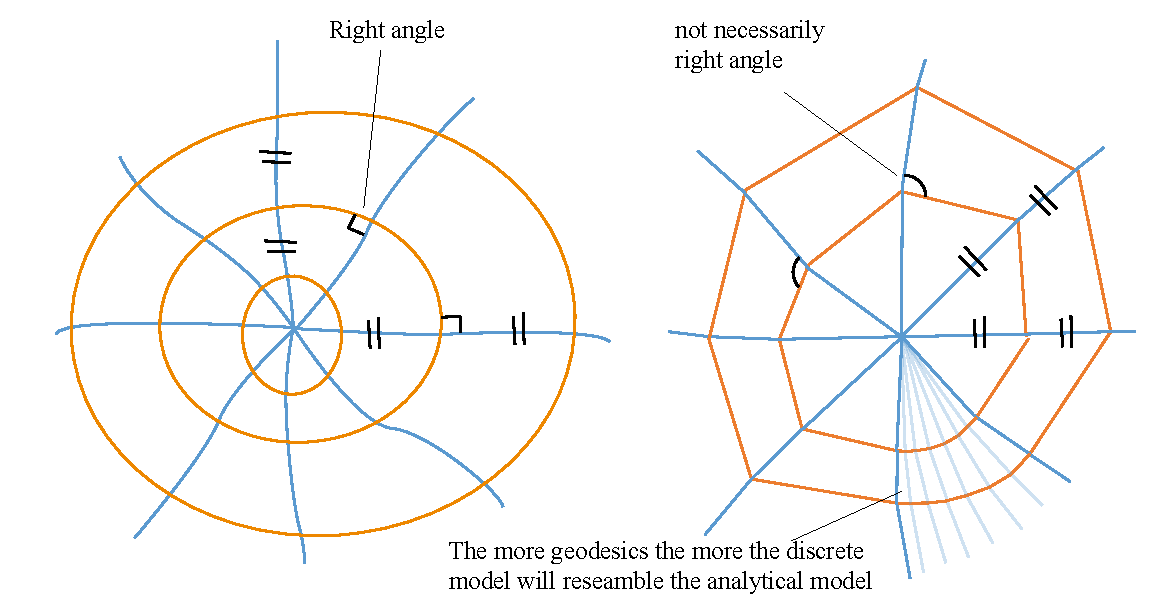
\includegraphics[width = 1.0\linewidth ]{figure/Method/polargeo.pdf}
\caption{To the right the continuos defition of polar geodesic coordinates and to the right a discrete interpretation. The discrete definition in this paper states that following continuous definition the discrete will at sufficient amount of sets of geodesic points the discrete will converge towards the continuous model}

\end{figure}

\subsubsection{Definition of discrete General Geodesic Coordinates}

For general geodesic coordinates it lacks a common starting points for the geodesics. It is therefore necessary to add a condition to the one of equal length. The angles that are created when two adjacent points from two sets geodesic points are of similar angle $\alpha$ , see figure below, it will resemble a orthogonal trajectory, and fore an infinite amounts of geodesics sets it will be continuous orthogonal trajectory. Finding one discrete line that fulfills the definition above ensures that the next discrete orthogonal trajectory can be found an equal distance spacing of the geodesic points.

\begin{figure}[H]
\centering
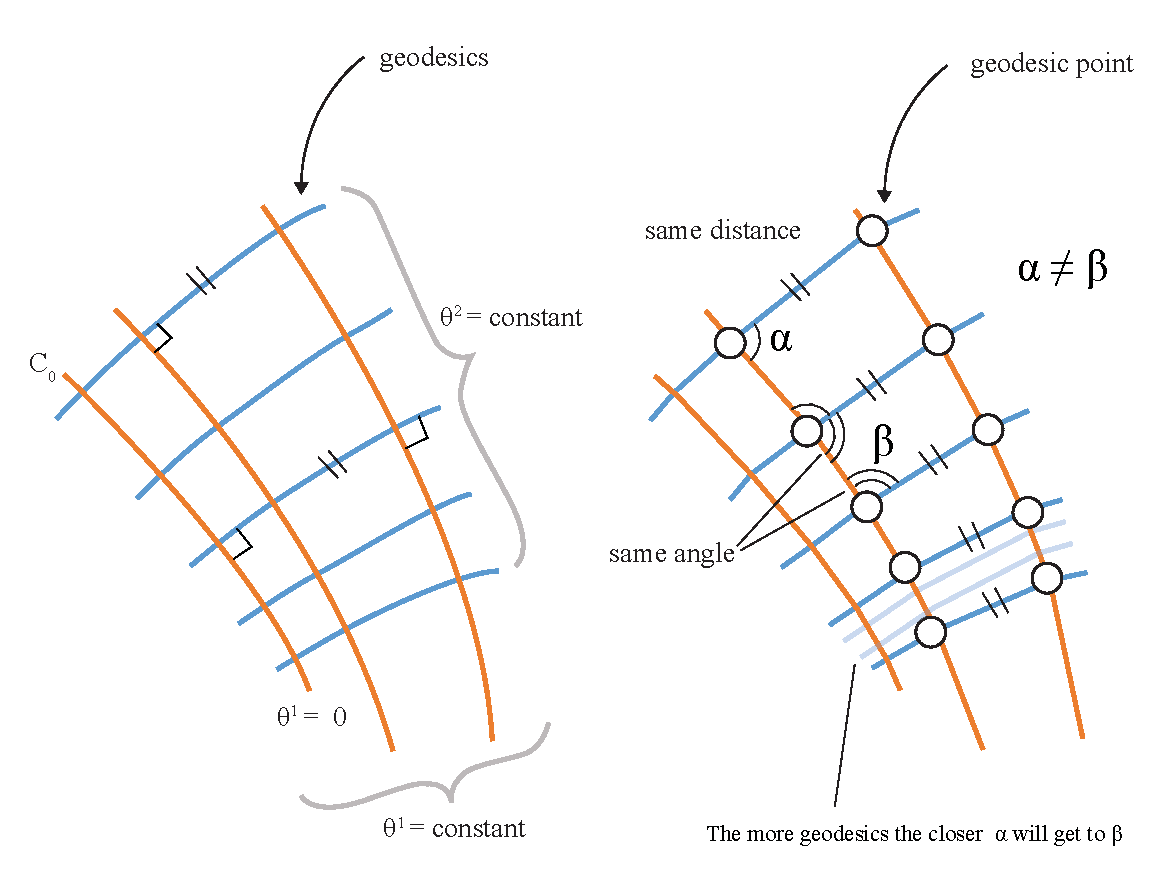
\includegraphics[width = 1.0\linewidth ]{figure/Method/diiscreteGeodesicCoord.pdf}
\caption{To the right the continuos defition of polar geodesic coordinates and to the right a discrete interpretation. The discrete definition in this paper states that following continuous definition the discrete will at sufficient amount of sets of geodesic points the discrete will converge towards the continuous model}
\label{fig:geoGen}
\end{figure}




\section{Separated form and geodesic generation}

This method as it states separate the form generation and the geodesic pattern generation. Therefore it gives more freedom in the sense that the form-generation can be focused on spatial and structural requirements. The method can be divided into three different stages.

\begin{enumerate}
\item Generate a form that satisfies equilibrium for masonry structures
\item Generate geodesics, that does not cross each other, on that surface
\item Generate the orthogonal trajectories that cuts the geodesics in equal length curves. 
\end{enumerate}

\subsection{Model preparation and Form-finding}


For this purpose it is only interesting to use numerical form-finding methods. It should be possible to choose whichever that pleases you where you can apply vertical loads for self-weight. For masonry structures it is important though that all forces and stresses acts in compression. The most suitable method for masonry structures is the TNA but it not implemented in a parametric environment, so far, so in this case traditional FD or DR method will be used. The numerical solvers implemented generates a set of curves or a mesh. To generate a surface from this a standard feature in \textit{Grasshoper3d} is used to convert a discrete surface to a mathematical surface.



\begin{figure}[H]
\centering
\includegraphics[width = 1.0\linewidth ]{figure/Method/ModelGen.jpg}
\end{figure}



\subsection{Generation of Geodesic Coordinates}

The geodesic coordinates generation will be based on the physical definition of the geodesic points. This is possible to model using DR or PS. The geodesic coordinates will be based on a generation of geodesic points that satisfies the discrete definitions of each coordinate system.\\
The process will be different for each case of geodesic coordinates. The Polar Geodesic Coordinates it is sufficient to only generate the geodesic points to satisfy the discrete definition. For the general geodesic coordinates one must combine the generation of geodesic points with the angle condition described in the definition. This will be described more in detail in the sections below.



\subsubsection{Polar Geodesic Coordinates}

The main idea of this method is to generate geodesic points that are equally spaced with a certain distance for all sets of points. This will be done using a DR solver modelling the set of points as discrete curves of springs on the surface. This is possible due to the physical definition in \ref{physdef}. 

The physical modelling requires the following:
\begin{enumerate}
\item The end points of the discrete curves are fixed and are allowed to rotate.
\item The initial springs should be modelled with equal length. It is important that the curves does not cross each other.
\item All members should have the same stiffness
\item The pretension force applied in the springs should be equal.
\end{enumerate}

The second and third statement makes it easy to impose forth statement. If all these are true the DR should result in equally spaced geodesic points between the two end points.

\vspace{5mm}

The Procedure can be described as following:

\begin{enumerate}
\item Decide the start and end points of the geodesics on the surface.
\item Generate an initial curve that lies on the surface based on the start and end points.
\item Discretize  the curve into segments, small enough to resemble the curve properties, of the same length. These segments will be modelled as springs in physical model where the springs have the same stiffness.
\item Apply the same pretension in all elements and ensure that the nodes move along the surface, this can be done by either a force or just moving the point to surface in each iteration. 
\item Start the solver, and for each iteration check the geodesic requirement for each point, or node. When all nodes are geodesic points then solution has converged and the iterations end. The geodesic points should, due to the equal initial length and tension, still have equal distance. 

\end{enumerate}

\begin{figure}[H]
\centering
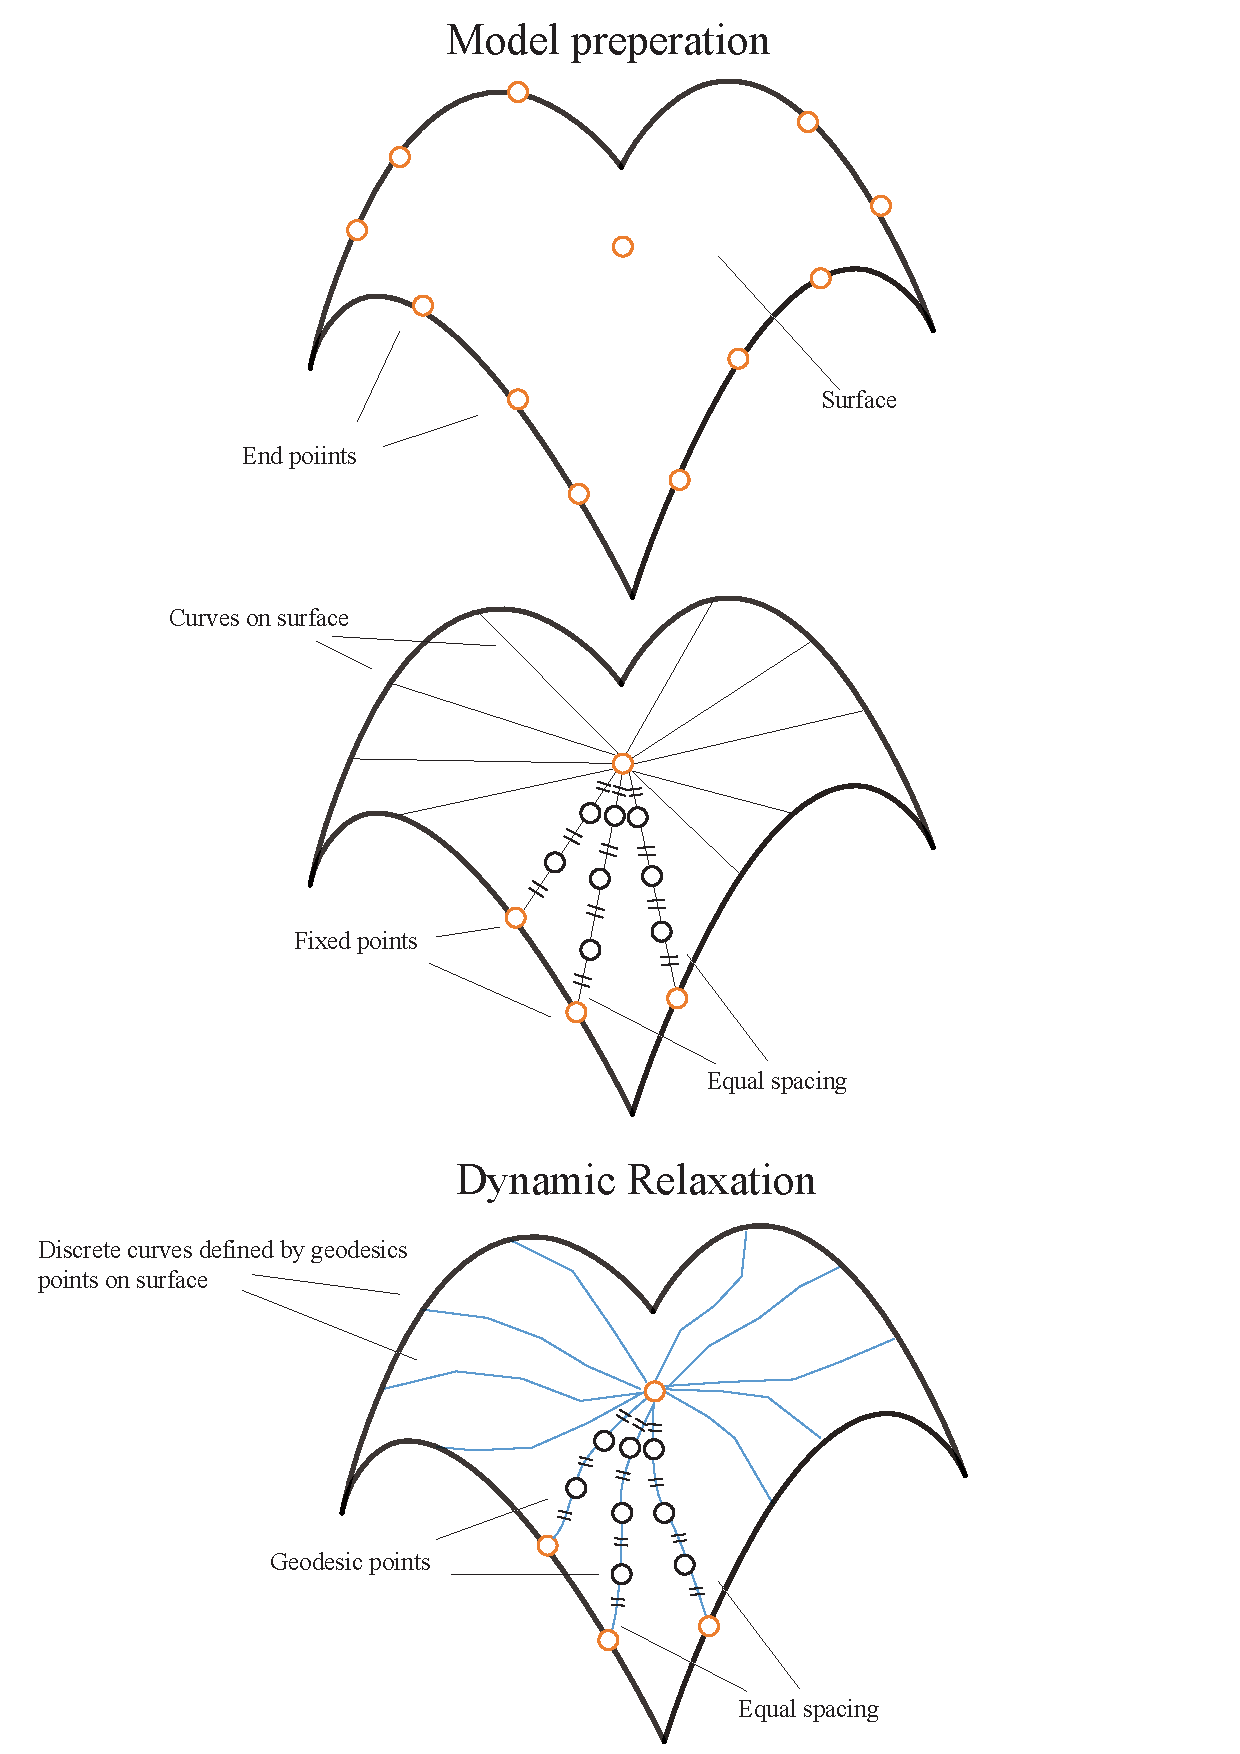
\includegraphics[width = 1.0\linewidth ]{figure/Method/Stepps.pdf}

\end{figure}

\subsubsection{General Geodesic Coordinates}

The main idea of this method is to generate geodesic points where one discrete curve connecting the geodesic sets has the same angle, see figure below. This discrete curve will be the reference, similar as the pole that will guarantee the discrete geodesic coordinate condition, meaning at an equal distance we will find the next orthogonal trajectory.

\begin{figure}[H]
\centering
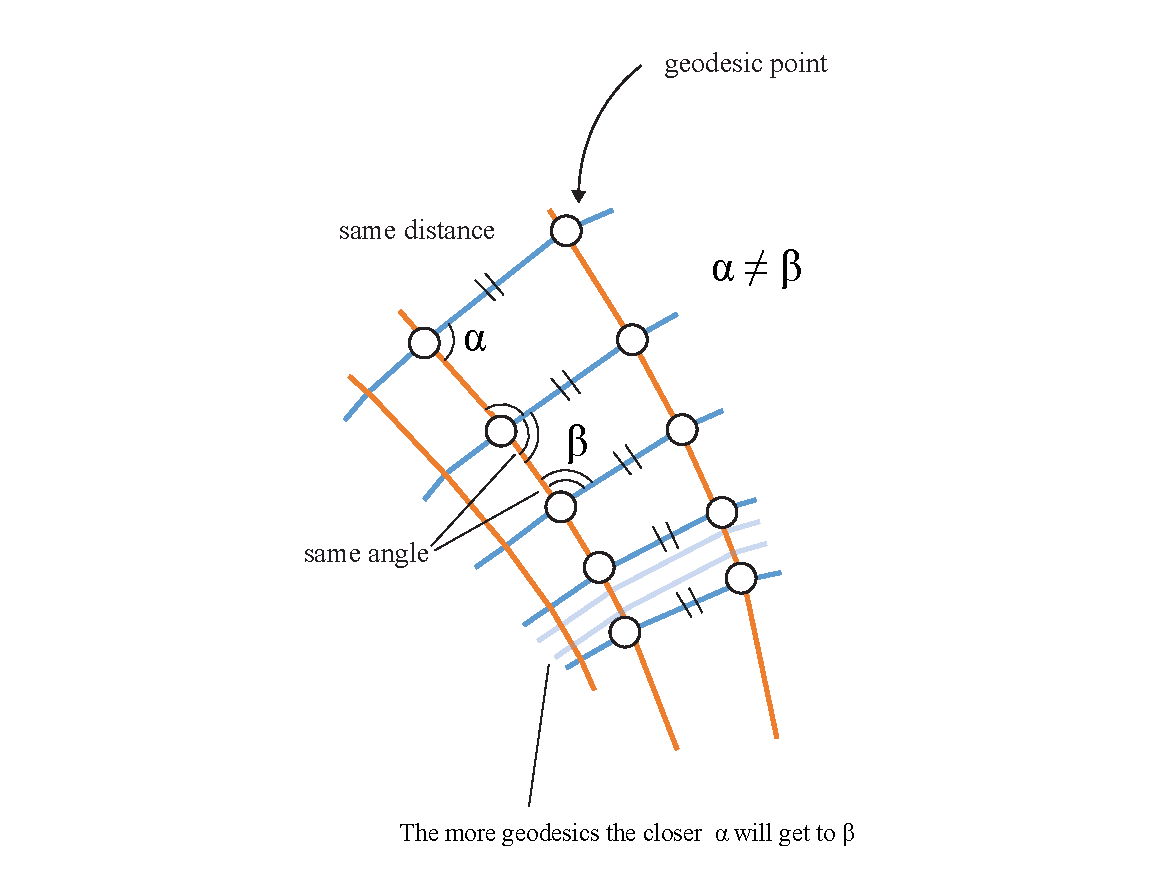
\includegraphics[width=0.9\linewidth ]{figure/Method/discreteGeodesicCoord2.pdf}
\caption{}
\end{figure}

The method of generating the geodesics cannot be made in as an simplistic manor as for polar coordinates. One must find geodesic points that are space equally that fulfills the definition above. Therefore it is not enough only finding these geodesics.

The physical mo

\begin{enumerate}
\item Decide the start and end points of the geodesics on the surface.
\item Generate an initial curve that lies on the surface based on the start and end points.
\item Discretize  the curve into segments, small enough to resemble the curve properties, of the same length. These segments will be modelled as springs in physical model. 
\item Separate the end springs on each sides and the middle springs. The middle springs should be modeled significantly stiffer then the ends.
\item Apply the same pretension in all elements and ensure that the nodes move along the surface, this can be done by either a force or just moving the point to surface in each iteration. 
\item Connect the angles $\alpha$ and $\beta$ to the stiffness of the end springs so that the end springs elongate and retract without changing the relation of the middle springs. 
\item Start the solver, and for each iteration check the geodesic requirement for each point, or node, and the angle between the geodesic sets. When these two conditions have been met the solution has converged and the iteration ends.
\end{enumerate}

The reason that the middle springs should be modeled significatly stiffer is because we want them to be equally spaced. The elongation and of the end springs will therefore not effect the middle springs.


 
\begin{figure}[H]
\centering
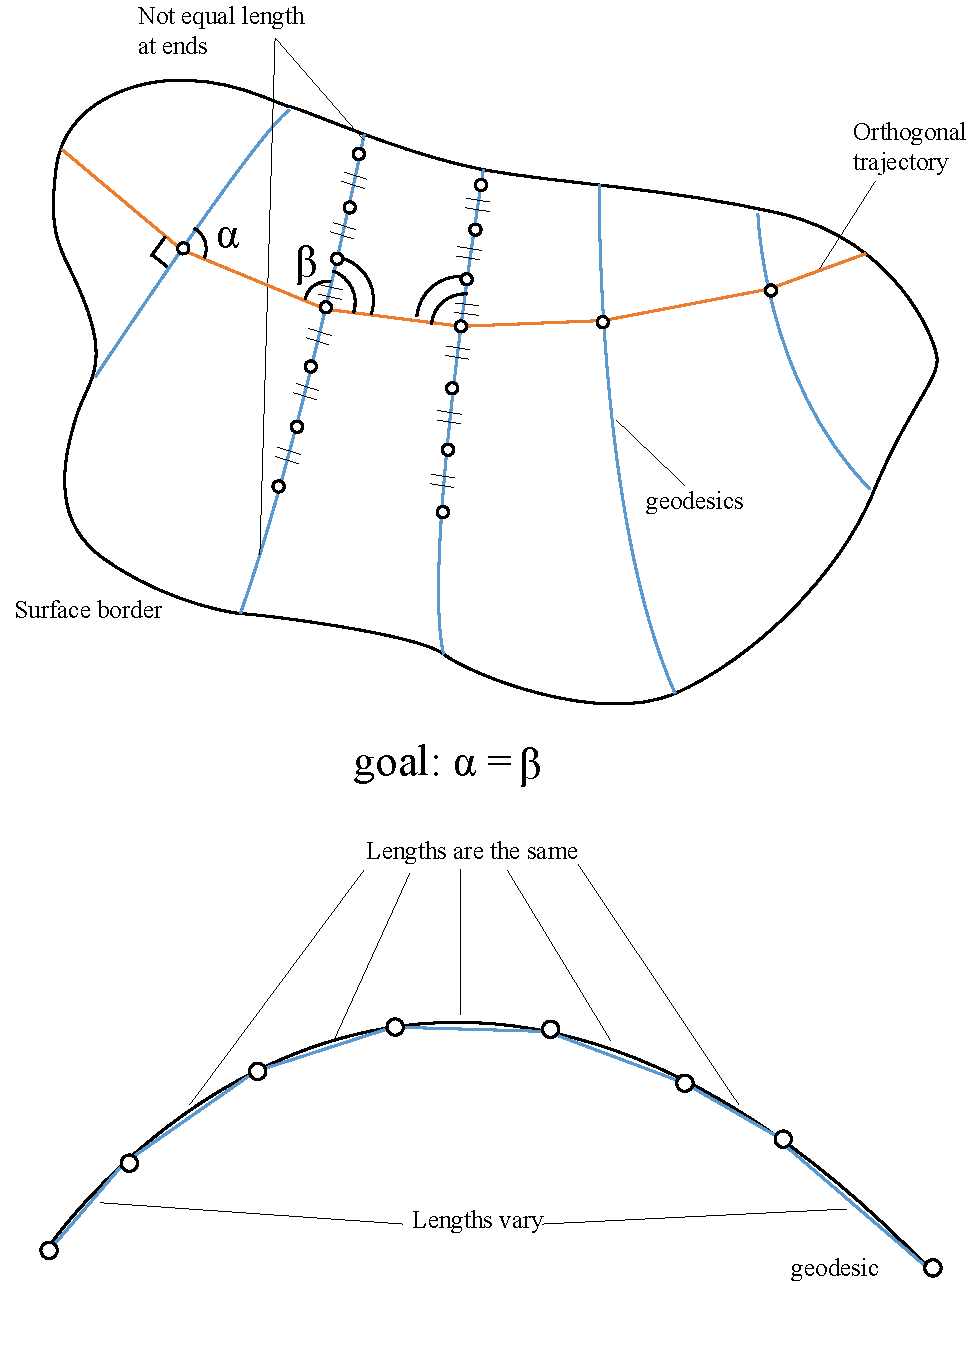
\includegraphics[width=0.9\linewidth ]{figure/Method/GeodesicCoord.pdf}
\caption{The fan vaults in Bath Abbey which has its own pole point in each fan vault.}
\end{figure}

